\documentclass[usenames,dvipsnames,tikz]{standalone}
\usetikzlibrary{patterns}
%\usetikzlibrary{shapes.geometric}
%\usepackage{xcolor}
\colorlet{tBlue}{RoyalBlue!35!Cerulean}
\colorlet{tRed}{Red}
%\definecolor{tGreen}{HTML}{569909}
%\definecolor{tOrange}{HTML}{FA7602}
\usepackage{tikz}
\usepackage{standalone}
\begin{document}	
	
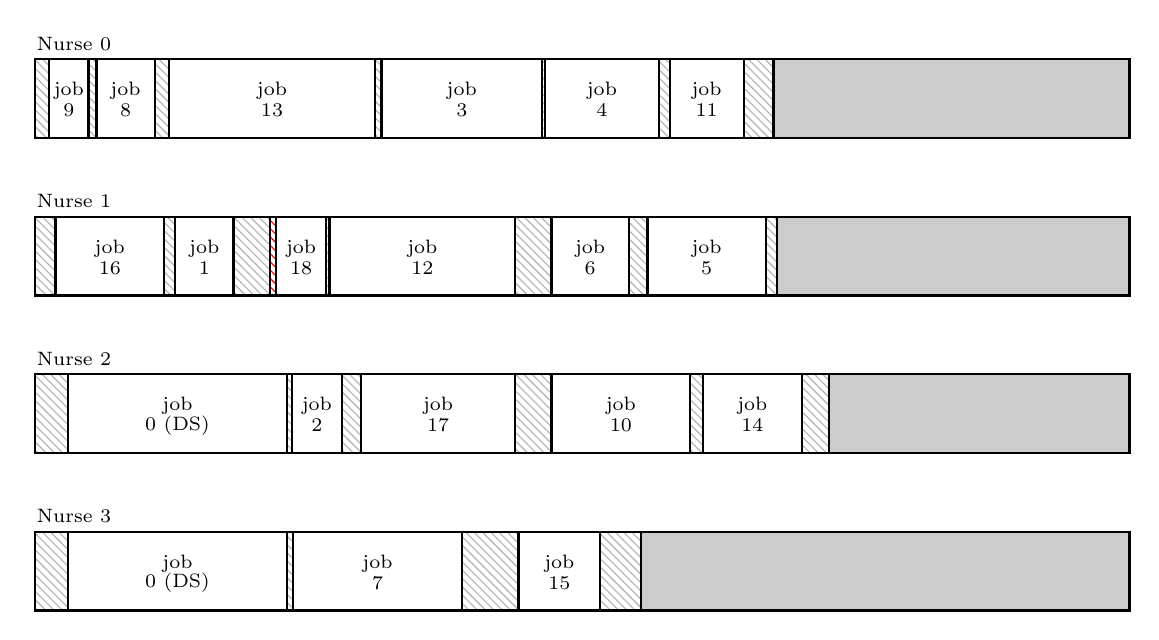
\begin{tikzpicture}
%\draw [help lines] (-1,-1) grid (15,8);

% Nurse 0
\draw [thick] (0,6) rectangle (13.9, 7);
\draw [thick, pattern = north west lines, pattern color=black!30!white] (0,6) rectangle (0.18,7);
\draw [thick] (0.18,6) -- (0.18,7); % start of job 9
\draw [thick] (0.68,6) -- (0.68,7); % end of job 9
\draw [thick, pattern = north west lines, pattern color=black!30!white] (0.68,6) rectangle (0.78,7);
\draw [thick] (0.78,6) -- (0.78,7); % start of job 8
\draw [thick] (1.52,6) -- (1.52,7); % end of job 8
\draw [thick, pattern = north west lines, pattern color=black!30!white] (1.52,6) rectangle (1.7,7);
\draw [thick] (1.7,6) -- (1.7,7); % start of job 13
\draw [thick] (4.32,6) -- (4.32,7); % end of job 13
\draw [thick, pattern = north west lines, pattern color=black!30!white] (4.32,6) rectangle (4.4,7);
\draw [thick] (4.4,6) -- (4.4,7); % start of job 3
\draw [thick] (6.44,6) -- (6.44,7); % end of job 3
\draw [thick, pattern = north west lines, pattern color=black!30!white] (6.44,6) rectangle (6.48,7);
\draw [thick] (6.48,6) -- (6.48,7); % start of job 4
\draw [thick] (7.92,6) -- (7.92,7); % end of job 4
\draw [thick, pattern = north west lines, pattern color=black!30!white] (7.92,6) rectangle (8.06,7);
\draw [thick] (8.06,6) -- (8.06,7); % start of job 11
\draw [thick] (9,6) -- (9,7); % end of job 11
\draw [thick, pattern = north west lines, pattern color=black!30!white] (9,6) rectangle (9.38,7);
\draw [thick] (9.38,6) -- (9.38,7); % end of shift
\draw [thick, fill=black!20!white] (9.38,6) rectangle (13.9,7);

\node [right] at (-0.1,7.2) {\scriptsize{Nurse 0}};
\node at (0.43,6.6) {\scriptsize{job}}; 
\node at (0.43,6.35) {\scriptsize{9}};
\node at (1.15,6.6) {\scriptsize{job}};
\node at (1.15,6.35) {\scriptsize{8}};
\node at (3.01,6.6) {\scriptsize{job}};
\node at (3.01,6.35) {\scriptsize{13}};
\node at (5.42,6.6) {\scriptsize{job}};
\node at (5.42,6.35) {\scriptsize{3}};
\node at (7.2,6.6) {\scriptsize{job}};
\node at (7.2,6.35) {\scriptsize{4}};
\node at (8.53,6.6) {\scriptsize{job}};
\node at (8.53,6.35) {\scriptsize{11}};


% Nurse 1
\draw [thick] (0,4) rectangle (13.9, 5);
\draw [thick, pattern = north west lines, pattern color=black!30!white] (0,4) rectangle (0.26,5);
\draw [thick] (0.26,4) -- (0.26,5); % start of job 16
\draw [thick] (1.64,4) -- (1.64,5); % end of job 16
\draw [thick, pattern = north west lines, pattern color=black!30!white] (1.64,4) rectangle (1.78,5);
\draw [thick] (1.78,4) -- (1.78,5); % start of job 1
\draw [thick] (2.52,4) -- (2.52,5); % end of job 1
\draw [thick, pattern = north west lines, pattern color=black!30!white] (2.52,4) rectangle (2.98,5);
\draw [thick] (2.98,4) -- (2.98,5); % ARRIVAL at job 18
\draw [thick, pattern = north west lines, pattern color=tRed] (2.98,4) rectangle (3.06,5);
\draw [thick] (3.06,4) -- (3.06,5); % start of job 18
\draw [thick] (3.7,4) -- (3.7,5); % end of job 18
\draw [thick, pattern = north west lines, pattern color=black!30!white] (3.7,4) rectangle (3.74,5);
\draw [thick] (3.74,4) -- (3.74,5); % start of job 12
\draw [thick] (6.10,4) -- (6.10,5); % end of job 12
\draw [thick, pattern = north west lines, pattern color=black!30!white] (6.10,4) rectangle (6.56,5);
\draw [thick] (6.56,4) -- (6.56,5); % start of job 6
\draw [thick] (7.54,4) -- (7.54,5); % end of job 6
\draw [thick, pattern = north west lines, pattern color=black!30!white] (7.54,4) rectangle (7.78,5);
\draw [thick] (7.78,4) -- (7.78,5); % start of job 5
\draw [thick] (9.28,4) -- (9.28,5); % end of job 5
\draw [thick, pattern = north west lines, pattern color=black!30!white] (9.28,4) rectangle (9.42,5);
\draw [thick] (9.42,4) -- (9.42,5); % end of shift
\draw [thick, fill=black!20!white] (9.42,4) rectangle (13.9,5);

\node [right] at (-0.1,5.2) {\scriptsize{Nurse 1}};
\node at (0.95,4.6) {\scriptsize{job}}; 
\node at (0.95,4.35) {\scriptsize{16}};
\node at (2.15,4.6) {\scriptsize{job}}; 
\node at (2.15,4.35) {\scriptsize{1}};
\node at (3.38,4.6) {\scriptsize{job}}; 
\node at (3.38,4.35) {\scriptsize{18}};
\node at (4.92,4.6) {\scriptsize{job}}; 
\node at (4.92,4.35) {\scriptsize{12}};
\node at (7.05,4.6) {\scriptsize{job}}; 
\node at (7.05,4.35) {\scriptsize{6}};
\node at (8.53,4.6) {\scriptsize{job}}; 
\node at (8.53,4.35) {\scriptsize{5}};


% Nurse 2
\draw [thick] (0,2) rectangle (13.9, 3);
\draw [thick, pattern = north west lines, pattern color=black!30!white] (0,2) rectangle (0.42,3);
\draw [thick] (0.42,2) -- (0.42,3); % start of job 0 (DS)
\draw [thick] (3.2,2) -- (3.2,3); % end of job 0 (DS)
\draw [thick, pattern = north west lines, pattern color=black!30!white] (3.2,2) rectangle (3.26,3);
\draw [thick] (3.26,2) -- (3.26,3); % start of job 2
\draw [thick] (3.9,2) -- (3.9,3); % end of job 2
\draw [thick, pattern = north west lines, pattern color=black!30!white] (3.9,2) rectangle (4.14,3);
\draw [thick] (4.14,2) -- (4.14,3); % start of job 17
\draw [thick] (6.1,2) -- (6.1,3); % end of job 17
\draw [thick, pattern = north west lines, pattern color=black!30!white] (6.1,2) rectangle (6.56,3);
\draw [thick] (6.56,2) -- (6.56,3); % start of job 10
\draw [thick] (8.32,2) -- (8.32,3); % end of job 10
\draw [thick, pattern = north west lines, pattern color=black!30!white] (8.32,2) rectangle (8.48,3);
\draw [thick] (8.48,2) -- (8.48,3); % start of job 14
\draw [thick] (9.74,2) -- (9.74,3); % end of job 14
\draw [thick, pattern = north west lines, pattern color=black!30!white] (9.74,2) rectangle (10.08,3);
\draw [thick] (10.08,2) -- (10.08,3); % end of shift
\draw [thick, fill=black!20!white] (10.08,2) rectangle (13.9,3);

\node [right] at (-0.1,3.2) {\scriptsize{Nurse 2}};
\node at (1.81,2.6) {\scriptsize{job}}; 
\node at (1.81,2.35) {\scriptsize{0 (DS)}};
\node at (3.58,2.6) {\scriptsize{job}}; 
\node at (3.58,2.35) {\scriptsize{2}};
\node at (5.12,2.6) {\scriptsize{job}}; 
\node at (5.12,2.35) {\scriptsize{17}};
\node at (7.44,2.6) {\scriptsize{job}}; 
\node at (7.44,2.35) {\scriptsize{10}};
\node at (9.11,2.6) {\scriptsize{job}}; 
\node at (9.11,2.35) {\scriptsize{14}};

% Nurse 3
\draw [thick] (0,0) rectangle (13.9, 1);
\draw [thick, pattern = north west lines, pattern color=black!30!white] (0,0) rectangle (0.42,1);
\draw [thick] (0.42,0) -- (0.42,1); % start of job 0 (DS)
\draw [thick] (3.20,0) -- (3.20,1); % end of job  0 (DS)
\draw [thick, pattern = north west lines, pattern color=black!30!white] (3.2,0) rectangle (3.28,1);
\draw [thick] (3.28,0) -- (3.28,1); % start of job 7
\draw [thick] (5.42,0) -- (5.42,1); % end of job 7
\draw [thick, pattern = north west lines, pattern color=black!30!white] (5.42,0) rectangle (6.14,1);
\draw [thick] (6.14,0) -- (6.14,1); % start of job 15
\draw [thick] (7.18,0) -- (7.18,1); % end of job 15
\draw [thick, pattern = north west lines, pattern color=black!30!white] (7.18,0) rectangle (7.7,1);
\draw [thick] (7.70,0) -- (7.70,1); % end of shift
\draw [thick, fill=black!20!white] (7.7,0) rectangle (13.9,1);

\node [right] at (-0.1,1.2) {\scriptsize{Nurse 3}};
\node at (1.81,0.6) {\scriptsize{job}}; 
\node at (1.81,0.35) {\scriptsize{0 (DS)}};
\node at (4.35,0.6) {\scriptsize{job}}; 
\node at (4.35,0.35) {\scriptsize{7}};
\node at (6.66,0.6) {\scriptsize{job}}; 
\node at (6.66,0.35) {\scriptsize{15}};






\end{tikzpicture}
	
\end{document}



